 \chapter{DISEÑO DE LA SOLUCIÓN PROPUESTA AL PROBLEMA CIENTÍFICO}
\label{chap:chapter2}


Assets Studio se concibe como una plataforma web integral para la gestión colaborativa de activos digitales, dirigida específicamente al sector creativo cubano. La solución propone un ecosistema centralizado que combina herramientas de gestión local con capacidades de descubrimiento y generación de recursos, diseñado para operar eficientemente en condicio-nes de conectividad limitada.
Sistema de Gestión de Usuarios y Colaboración

\begin{itemize}
    \item Implementación de perfiles multinivel (básico, avanzado, administrador)
    \item Sistema de comentarios y discusiones técnicas sobre assets
    \item Mecanismo de valoración mediante likes/favoritos
    \item Sistema de reportes para contenido inapropiado o mal etiquetado
    \item Historial de actividad y contribuciones comunitarias
\end{itemize}

Módulo de Descubrimiento y Adquisición de Assets

\begin{itemize}
    \item Scraping Ético a plataformas de recursos abiertos como OpenGameArt, con atribución automática de autoría
    \item Integración con APIs de generación de assets mediante IA para creación asistida
    \item Catálogo comunitario con filtros avanzados por licencia, formato y compatibilidad técnica
    \item Sistema de recomendaciones basado en el perfil de uso y preferencias
\end{itemize}

Gestión Integral de Activos Digitales

\begin{itemize}
    \item Subida Masiva de archivos con detección automática de metadatos
    \item Organización Inteligente mediante etiquetado automático asistido por IA
    \item Sistema de Versiones para tracking de modificaciones
    \item Descarga Selectiva con opciones de compresión adaptativa
    \item Almacenamiento Híbrido (local-nube) según criticidad y frecuencia de uso
\end{itemize}

Características Técnicas Especializadas
\begin{itemize}
    \item Previsualización en Tiempo Real de assets multiformato
    \item Conversión On-demand a formatos estándar de la industria
    \item Validación de Compatibilidad con motores gráficos y herramientas de diseño
    \item Sistema de Backup Automático con políticas de retención configurables
\end{itemize}

Arquitectura de Datos y Seguridad

\begin{itemize}
    \item Modelo de permisos granulares para trabajo colaborativo
    \item Encriptación punto a punto para assets sensibles
    \item Sistema de licencias y derechos de uso integrado
    \item Auditoría trazable de todas las operaciones realizadas
\end{itemize}

Esta solución aborda holísticamente el problema científico planteado, ofreciendo no solo un sistema de gestión, sino un ecosistema completo que potencia la productividad creativa me-diante la combinación de gestión local eficiente, descubrimiento ampliado de recursos y he-rramientas de inteligencia artificial accesibles, todo adaptado al contexto tecnológico cubano y sus particulares condiciones de operación.

\section{Epigrafe 1}
\subsection{ Modelado de los procesos de gestión y generación de activos digitales}

Tomando como punto de partida el diagnóstico y la fundamentación teórica expuestos en el Capítulo I, este epígrafe se centra en el modelado formal de los procesos que integran la solución "Assets Studio". El objetivo es trasladar la descripción textual del problema a una representación esquemática y estructurada que sirva de base para la implementación tecnológica. Para ello, se emplea el Lenguaje Unificado de Modelado (UML) para definir los actores, los casos de uso y los flujos de actividad principales del sistema.

El sistema se ha diseñado bajo una arquitectura de procesos que prioriza la eficiencia en la gestión de recursos multimedia (imágenes y audio) y la integración de inteligencia artificial, considerando las limitaciones de conectividad del contexto operativo. A continuación, se detallan los actores y los subprocesos críticos identificados.

\subsection{Identificación de Actores del Sistema}

Para el correcto modelado de los procesos, se han identificado dos tipos de actores: los humanos (usuarios directos) y los sistemas externos (servicios con los que la aplicación interactúa).


\begin{itemize}
    \item Usuario Invitado (No autenticado): Actor que accede a la plataforma con privilegios de solo lectura. Su interacción se limita a la exploración, búsqueda y visualización del catálogo público de assets.
    \item Usuario Registrado (Cliente): Actor principal del sistema. Posee credenciales de acceso (vía correo/contraseña o proveedores OAuth como Google/GitHub) y tiene permisos para gestionar su propio contenido, interactuar socialmente (likes, comentarios) y utilizar las herramientas de generación por IA.
    \item Administrador: Actor encargado de la moderación del contenido, gestión de reportes de abuso y supervisión de la integridad de los datos en la plataforma.
    \item Sistemas Externos:
    \begin{itemize}
        \item Cloudinary: Servicio encargado del almacenamiento físico y optimización de los assets.
        \item Firebase/Auth: Servicio encargado de la validación de identidad.
        \item API de IA: Servicio externo para la generación de imágenes a partir de prompts.
    \end{itemize}
\end{itemize}

\subsection{Modelado de Casos de Uso del Negocio}

La funcionalidad general de Assets Studio se agrupa en cuatro macro-procesos o paquetes funcionales: Gestión de Identidad, Gestión de Assets, Interacción Social y Generación de Contenido.

[Figura II.1. Diagrama de Casos de Uso General del Sistema]
(Nota para el estudiante: En este diagrama debes mostrar al Usuario Registrado conectado con óvalos que digan "Subir Asset", "Generar Asset con IA", "Comentar", "Dar Like", "Gestionar Perfil". El Usuario Invitado solo debe conectar con "Buscar Asset" y "Visualizar Asset").

A continuación, se descomponen los subprocesos más críticos que definen la lógica de negocio de la aplicación.

\subsection{Subproceso de Publicación y Gestión de Assets}

Este es el proceso central de la plataforma. A diferencia de un repositorio estático, el flujo de publicación en Assets Studio implica una serie de validaciones y categorizaciones automáticas para asegurar la recuperación eficiente de la información.

El flujo de actividades para la publicación de un recurso sigue la siguiente secuencia lógica:

    \begin{itemize}
        \item Solicitud de carga: El usuario selecciona uno o varios archivos (imágenes o audio).
        \item Validación preliminar: El sistema verifica en el cliente el formato y peso del archivo.
        \item Procesamiento externo: El archivo es enviado a Cloudinary, donde se almacena y se generan las variantes necesarias (miniaturas, formatos optimizados).
        \item Registro de Metadatos: Una vez confirmada la subida, el sistema registra en la base de datos (PostgreSQL/Neon) la URL del recurso, asignándole automáticamente la categoría seleccionada por el usuario y procesando las etiquetas (tags) para la búsqueda semántica.
        \item Vinculación: El asset se asocia al ID del usuario creador y se publica en el feed general.
    \end{itemize}

    [figura: Figura II.2. Diagrama de Actividad del Proceso de Subida de Assets]
    (Nota: Dibuja un diagrama de flujo donde se vea: Inicio -> Seleccionar Archivo -> ¿Es válido? (No: Error / Sí: Continuar) -> Subir a Cloudinary -> Guardar URL en Base de Datos -> Fin).

\subsection{Subproceso de Generación de Contenido Asistido por IA}

Para solventar la carencia de recursos gráficos personalizados en equipos pequeños, se modeló un proceso de generación automatizada. Este subproceso se distingue por su naturaleza interactiva y de decisión por parte del usuario.

El modelo del proceso es el siguiente:

\begin{itemize}
        \item Entrada de Datos: El usuario introduce una descripción textual (prompt) de lo que desea generar.
        \item Procesamiento: El sistema envía la solicitud a la API de Inteligencia Artificial.
        \item Revisión: El sistema presenta el resultado generado al usuario de forma temporal.
        \item Decisión: El usuario tiene tres opciones:
         \begin{itemize}
            \item Descartar: Se elimina la imagen temporal y se reinicia el proceso.
            \item Descargar: Se guarda localmente sin registrarse en la plataforma.
            \item Publicar/Guardar: Se inicia el subproceso de "Gestión de Assets" descrito anteriormente para integrarlo en su perfil.
        \end{itemize}
\end{itemize}

\subsection{Subproceso de Interacción y Notificaciones}

Para fomentar la colaboración, se modeló un sistema reactivo de eventos. Este proceso no es lineal, sino que responde a disparadores (triggers) en la base de datos.

\begin{itemize}
        \item Evento: Un usuario realiza una acción sobre un asset ajeno (Comentario o Like).
        \item Persistencia: Se guarda la relación en las tablas Coment o Like.
        \item Disparo de Notificación: El sistema identifica al propietario del asset y genera un registro en la tabla Notifications.
        \item Entrega: La próxima vez que el usuario propietario actualice su estado o navegue por la web, el sistema consulta las notificaciones no leídas y alerta visualmente al usuario.
\end{itemize}

\section{Emigrafe 2}
\subsection{ Ingeniería de Requisitos, Análisis y Diseño de la Solución}

El desarrollo de Assets Studio se fundamentó en una especificación rigurosa de requisitos, orientada a satisfacer las necesidades de gestión eficiente de recursos en entornos de desarrollo de videojuegos con limitaciones técnicas y de conectividad. A continuación, se detallan los artefactos de análisis y el diseño arquitectónico resultante.

\subsection{ Requisitos Funcionales del Sistema (RF)}

Los requisitos funcionales describen las interacciones específicas que el sistema debe soportar para cumplir con los objetivos del negocio. Se han clasificado según los módulos principales de la aplicación:

Módulo de Gestión de Identidad y Seguridad:
\begin{itemize}
    \item RF-01 Autenticación: El sistema debe permitir el registro e inicio de sesión mediante correo electrónico/contraseña y proveedores externos (Google y GitHub) utilizando Firebase Authentication.
    \item RF-02 Gestión de Perfil: El usuario autenticado debe poder modificar su avatar, nombre visible y contraseña.
    \item RF-03 Roles de Usuario: El sistema debe diferenciar entre usuarios con rol client (acceso estándar) y admin (moderación y gestión), tal como se define en el esquema de datos.
\end{itemize}

Módulo de Gestión de Activos (Assets):
    \begin{itemize}
        \item RF-04 Carga de Recursos: El sistema debe permitir la subida de archivos de imagen y audio, validando formatos y tamaños antes de su almacenamiento en Cloudinary.
        \item RF-05 Categorización: Todo activo debe ser clasificado obligatoriamente en categorías predefinidas (Object, Character, Nature, City, Surfaces, Other) y etiquetado con tags para su recuperación.
        \item RF-06 Visualización y Descarga: Los usuarios (autenticados o no) deben poder visualizar los detalles del asset y descargarlo en su formato original.
        \item RF-07 Generación con IA: El sistema debe proveer una interfaz para ingresar prompts de texto y recibir imágenes generadas artificialmente, permitiendo su guardado directo en la biblioteca del usuario.
    \end{itemize}

    Módulo de Interacción Social:
      \begin{itemize}
        \item RF-08 Feedback: Los usuarios deben poder comentar y valorar ("dar like") los activos de otros usuarios.
        \item RF-09 Sistema de Reportes: Se debe permitir reportar contenido inapropiado (Spam, Abuse, Fraud, etc.) para su posterior revisión.
        \item RF-10 Notificaciones: El sistema debe notificar al autor cuando su contenido recibe interacción (likes o comentarios).
    \end{itemize}

    \subsection{Requisitos No Funcionales (RNF)}

    Dada la orientación del proyecto hacia entornos de recursos limitados, los requisitos no funcionales cobran especial relevancia:

    \begin{itemize}
        \item RNF-01 Optimización de Carga: Las imágenes deben servirse en formatos optimizados (WebP/AVIF) y redimensionadas según el dispositivo del usuario para minimizar el consumo de ancho de banda.
        \item RNF-02 Escalabilidad de Base de Datos: La persistencia de datos debe gestionarse mediante una arquitectura Serverless (Neon PostgreSQL) que soporte picos de concurrencia sin degradación del servicio.
        \item RNF-03 Rendimiento de Interfaz: La aplicación debe utilizar renderizado híbrido (SSR/CSR) proporcionado por Next.js para asegurar tiempos de primera pintura (FCP) inferiores a 1.5 segundos.
        \item RNF-04 Integridad de Datos: El sistema debe garantizar la consistencia referencial entre los usuarios, sus activos y las interacciones asociadas mediante el uso del ORM Prisma.
    \end{itemize}

\subsection{Arquitectura del Sistema}

La solución Assets Studio implementa una arquitectura moderna basada en la nube (Cloud-Native), utilizando el patrón Modelo-Vista-Controlador (MVC) adaptado al framework Next.js. Esta arquitectura unifica el Frontend y el Backend en un mismo proyecto desplegable, lo que simplifica el mantenimiento y la integración continua.

La arquitectura se divide en tres capas lógicas:

    \begin{itemize}
        \item Capa de Presentación (Frontend): Construida con React.js, es responsable de la interfaz de usuario y la interacción directa. Se comunica con la capa de servicios a través de llamadas API internas.
        \item Capa de Aplicación y Servicios (Backend/API): Gestionada por los API Routes de Next.js. Aquí reside la lógica de negocio, la validación de sesiones con Firebase Admin y la orquestación de llamadas a servicios externos (IA y Cloudinary).
        \item Capa de Persistencia (Datos):
            \begin{itemize}
               \item Almacenamiento Estructurado: Base de datos PostgreSQL alojada en Neon, gestionada mediante Prisma ORM para operaciones CRUD seguras y tipadas.
               \item Almacenamiento de Blobs: Cloudinary se utiliza como repositorio de objetos para los archivos multimedia (imágenes y audio), almacenando en la base de datos únicamente las referencias (URLs públicas y IDs).
             \end{itemize}

    \end{itemize}

[Figura II.3. Diagrama de Arquitectura del Sistema]
(Nota para el estudiante: Dibuja un diagrama de bloques. Al centro pon "Next.js App (Frontend + API)". Con flechas bidireccionales conéctalo a: "Neon (PostgreSQL)" abajo, "Cloudinary" a la derecha, "Firebase Auth" a la izquierda y "IA Service" arriba).

\subsection{Diseño del Modelo de Datos}

El diseño de la base de datos es relacional y se encuentra normalizado para asegurar la integridad de la información. El modelo se implementó utilizando el esquema de Prisma, definiendo las siguientes entidades principales:

    \begin{itemize}
        \item User: Entidad central que almacena credenciales, roles  y referencias a proveedores de identidad.
        \item Asset: Representa el recurso digital. Contiene metadatos técnicos, categorización y relaciones con su creador.
        \item AssetImage / AssetTag: Entidades auxiliares para gestionar propiedades específicas de las imágenes y el sistema de etiquetado para búsquedas.
        \item Interacciones (Like, Coment, Report): Tablas relacionales que vinculan usuarios con activos, permitiendo la trazabilidad de la actividad social.
        \item Notifications: Entidad transaccional diseñada para gestionar la comunicación asíncrona con el usuario sobre eventos relevantes.
    \end{itemize}

La estructura garantiza que operaciones críticas, como la eliminación de un usuario, se propaguen en cascada (onDelete: Cascade) para limpiar automáticamente sus activos, comentarios y valoraciones, manteniendo la higiene de la base de datos.

[Figura II.4. Diagrama Entidad-Relación (DER)]
(Nota: Aquí puedes usar una captura del diagrama que genera Prisma Studio o dibujar el esquema de tablas: User 1---N Asset, Asset 1---N Like, Asset 1---N Coment, etc. Asegúrate de mostrar las claves foráneas).

\section{Epigrafe 3}
\subsection{Diseño de mecanismos de datos, implementación e interfaces de usuario}

La eficiencia operativa de Assets Studio reside en su capacidad para gestionar grandes volúmenes de datos multimedia sin comprometer el rendimiento del cliente final. Para ello, se diseñó una arquitectura de datos híbrida que separa el almacenamiento de metadatos relacionales del almacenamiento de objetos binarios (BLOBs), optimizando tanto la transmisión como el procesamiento.

\subsection{Mecanismos de Almacenamiento y Persistencia}

La estrategia de persistencia se implementó siguiendo un modelo distribuido para garantizar la escalabilidad y la integridad referencial:
    \begin{itemize}
        \item Almacenamiento Relacional (Metadatos): Se utilizó PostgreSQL desplegado en Neon (Serverless). Este mecanismo gestiona la estructura lógica del negocio: usuarios, relaciones sociales (likes, comentarios), y los punteros a los archivos. La interacción con la base de datos se abstrae mediante el ORM Prisma, lo que permite definir un esquema tipado y seguro.
        \item Almacenamiento de Objetos (Media): Los archivos pesados (imágenes y audio) se delegan a Cloudinary. Esta plataforma no solo almacena el archivo raw, sino que realiza transformaciones automáticas (formato, calidad, redimensionamiento) antes de entregarlo al cliente, cumpliendo con el requisito de optimización de ancho de banda.
    \end{itemize}

El siguiente fragmento de código muestra la definición del esquema en Prisma (schema.prisma) utilizado para vincular ambas fuentes de datos, donde el modelo Asset almacena la referencia src proveniente de la nube y la relaciona con el usuario y las interacciones locales:

codePrisma

% // Implementación del Modelo de Datos en Prisma (Fragmento)
% model Asset {
%   id          Int      @id @default(autoincrement())
%   src         String   // URL del recurso en Cloudinary
%   public_id   String   // Identificador único del archivo
%   format      String   // Formato optimizado (ej. webp, avif)
%   user_id     String
%   categoria   String   @default("other")
%   createdAt   DateTime @default(now())
  
%   // Relaciones de Integridad Referencial
%   likes       Like[]
%   coments     Coment[]
%   tags        AssetTag[]
%   image       AssetImage?
% }

% model AssetTag {
%   id     Int    @id @default(autoincrement())
%   name   String @unique 
%   assets Asset[]
% }

\subsection{Mecanismos de Procesamiento y Transmisión}
La transmisión de datos entre el cliente (navegador) y el servidor se realiza mediante API Routes de Next.js, utilizando el protocolo HTTPS y el formato JSON para el intercambio de mensajes.

El flujo de procesamiento para la creación de un nuevo asset (ya sea subido o generado por IA) sigue una lógica transaccional para evitar datos huérfanos:
    \begin{itemize}
        \item Validación de Sesión: Se verifica el token de autenticación del usuario (Firebase).
        \item Carga/Generación: El archivo se procesa y se sube a Cloudinary.
        \item Transacción de Base de Datos: Una vez obtenida la URL segura, se ejecuta una operación de escritura en PostgreSQL.
    \end{itemize}

A continuación, se presenta un ejemplo de la lógica de implementación utilizada en el controlador del backend para registrar un asset, asegurando que se guarden tanto la imagen como sus etiquetas asociadas:

codeJavaScript

% // Lógica de Controlador para la Creación de Assets (Pseudocódigo)
% export async function POST(request) {
%   const body = await request.json();
%   const { src, public_id, format, tags, userId, category } = body;

%   try {
%     const newAsset = await prisma.asset.create({
%       data: {
%         src,
%         public_id,
%         format,
%         user_id: userId,
%         categoria: category,
%         // Conexión o creación de etiquetas en la misma transacción
%         tags: {
%           connectOrCreate: tags.map((tag) => ({
%             where: { name: tag },
%             create: { name: tag },
%           })),
%         },
%       },
%     });
%     return NextResponse.json(newAsset);
%   } catch (error) {
%     return NextResponse.json({ error: "Error en persistencia" }, { status: 500 });
%   }
% }

\subsection{Diseño de Interfaces Gráficas de Usuario (GUI)}

a interfaz de usuario se diseñó priorizando la usabilidad y la carga progresiva (Lazy Loading). Se implementó un diseño responsivo que se adapta a dispositivos móviles y de escritorio, utilizando una paleta de colores oscuros para resaltar el contenido visual (los assets) y reducir la fatiga visual en sesiones de trabajo prolongadas.

Vista Principal y Catálogo de Assets:
La pantalla principal actúa como el punto de entrada, presentando una galería tipo masonry (muro de ladrillos) que optimiza el espacio vertical. Incluye una barra de búsqueda semántica y filtros por categoría.

[Figura II.5. Interfaz de la Página Principal y Galería de Assets]
(Nota: Captura de pantalla donde se vea la barra de búsqueda arriba y la cuadrícula de imágenes abajo).

Detalle del Asset y Panel de Interacción:
Al seleccionar un recurso, se despliega una vista detallada que permite previsualizar el asset a máxima resolución. En esta interfaz se integran los componentes sociales: botón de "Me gusta", sección de comentarios en tiempo real y opciones de descarga.

[Figura II.6. Interfaz de Detalle de Asset con Comentarios y Opciones]
(Nota: Captura donde se vea una imagen grande, y al lado o abajo los comentarios de usuarios y el botón de descarga).

Panel de Gestión y Generación con IA:
Esta interfaz permite al usuario autenticado subir sus propios archivos o utilizar la herramienta de generación. Se diseñó un formulario intuitivo que guía al usuario en el etiquetado del recurso. En el caso de la IA, incluye un campo de texto para el prompt y un área de previsualización para decidir si descartar o guardar el resultado.

[Figura II.7. Interfaz de Generación de Assets mediante IA]
(Nota: Captura del formulario donde pones el texto para la IA y te muestra la imagen generada).

\section{Epigrafe 4}
\subsection{Diseño de la gestión de errores y despliegue de la solución}

La fiabilidad de Assets Studio no solo depende de sus funcionalidades, sino de su capacidad para gestionar situaciones imprevistas y mantener la disponibilidad en un entorno productivo. En este epígrafe se detalla la estrategia de tolerancia a fallos y el diseño de la arquitectura de despliegue en la nube.

\subsection{Estrategia de Gestión y Tratamiento de Errores}

El sistema implementa una estrategia de "defensa en profundidad" para el manejo de excepciones, abordando los errores en tres niveles: interfaz de usuario, lógica de servidor y base de datos.

Nivel de Interfaz (Frontend):
    \begin{itemize}
        \item Validación Preventiva: Se implementaron validaciones de formulario en tiempo real para evitar el envío de datos incorrectos (ej. formatos de archivo no soportados o campos vacíos).
        \item Feedback Visual: Ante fallos en la carga de assets o errores de red, el sistema despliega notificaciones tipo Toast (alertas emergentes) que informan al usuario del estado de la operación sin interrumpir su navegación.
        \item Páginas de Error (Fallbacks): Se diseñaron páginas estáticas personalizadas (404 Not Found y 500 Server Error) para mantener la identidad visual de la marca incluso cuando el servidor no responde.
    \end{itemize}

Nivel de Servidor y API (Backend):
     \begin{itemize}
        \item Bloques Try/Catch: Todas las rutas de la API (Next.js API Routes) envuelven sus operaciones críticas en bloques de manejo de excepciones. Esto asegura que si falla un servicio externo (como Cloudinary o la IA), el servidor no se detenga, sino que devuelva un código HTTP adecuado (ej. 503 Service Unavailable o 400 Bad Request).
        \item Manejo de Errores de Base de Datos: Prisma ORM gestiona los errores de conexión con Neon. Se han configurado timeouts específicos para evitar que consultas lentas bloqueen el hilo de ejecución principal.
    \end{itemize}

Reporte Participativo de Errores:

     \begin{itemize}
        \item Aprovechando el modelo de datos Report definido en el esquema, se habilitó un mecanismo para que los usuarios finales reporten anomalías.
        \item Los usuarios pueden señalar assets corruptos o fallos funcionales, creando un registro directo en la base de datos para su posterior revisión por un administrador.
    \end{itemize}

[Figura II.8. Diagrama de Flujo de Gestión de Excepciones]
(Nota para el estudiante: Dibuja un diagrama sencillo: Usuario realiza acción -> ¿Error en datos? (Sí: Mensaje de alerta / No: Enviar al Servidor) -> Servidor procesa -> ¿Fallo externo? (Sí: Retornar error 500 / No: Éxito). Incluye una cajita que diga "Registro en Log").

\subsection{Diseño del Despliegue (Deployment)}

La arquitectura de despliegue de Assets Studio sigue un modelo Serverless y distribuido, diseñado para maximizar la disponibilidad y minimizar los costes de mantenimiento de infraestructura. La solución se despliega aprovechando la integración nativa del ecosistema Next.js.

El flujo de despliegue continuo (CI/CD) consta de las siguientes etapas:

     \begin{itemize}
        \item Entorno de Desarrollo Local: Los desarrolladores trabajan sobre ramas de características (feature branches), ejecutando la aplicación en un entorno Node.js local que conecta con una base de datos de desarrollo en Neon.
        \item Control de Versiones: El código se gestiona en un repositorio remoto (GitHub).
        \item Build y Despliegue Automático:
            \begin{itemize}
                \item Al realizar un push a la rama principal (main), se dispara el proceso de construcción (build) en la plataforma de hosting (Vercel).
                \item Durante el build, Next.js optimiza las imágenes, compila las rutas estáticas y verifica las dependencias.
                \item Las migraciones de base de datos (prisma migrate deploy) se ejecutan para asegurar que el esquema en Neon coincida con la nueva versión del código.
            \end{itemize}
        \item Producción: Una vez finalizado el proceso, la nueva versión se distribuye automáticamente a través de una red de entrega de contenido (CDN) global.
    \end{itemize}

Componentes de la Infraestructura de Producción: la Infraestructura de Producción: la Infraestructura de Producción: la Infraestructura de Producción: la Infraestructura de Producción: la Infraestructura de Producción: la Infraestructura de Producción: la Infraestructura de Producción:
    \begin{itemize}
        \item Servidor Web/App: Vercel (Ejecución de Next.js y Serverless Functions).
        \item Base de Datos: Neon (PostgreSQL gestionado).
        \item Almacenamiento Media: Cloudinary (CDN para imágenes y audio).
        \item Autenticación: Firebase Identity Platform.
    \end{itemize}

[Figura II.9. Diagrama de Despliegue de la Solución]
(Nota: Dibuja un diagrama de despliegue UML. Muestra nodos (cubos 3D): "Cliente (Navegador)", "Servidor de Aplicaciones (Vercel)", "Servidor de Base de Datos (Neon)", "Servidor de Archivos (Cloudinary)". Conecta los nodos con líneas que indiquen el protocolo, ej: "HTTPS/JSON").

\subsection{Gestión de Variables de Entorno y Seguridad}

Para garantizar la seguridad del despliegue, ninguna credencial se almacena en el código fuente. Se utiliza un sistema de variables de entorno (.env) inyectadas en tiempo de ejecución. Las variables críticas configuradas en el entorno de producción incluyen:

    \begin{itemize}
        \item DATABASE URL: Cadena de conexión encriptada a la instancia de Neon.
        \item NEXT PUBLIC CLOUDINARY CLOUD NAME: Identificador público para la carga de imágenes.
        \item CLOUDINARY API SECRET: Llave privada para firmar las subidas de archivos (backend).
        \item FIREBASE CLIENT EMAIL y PRIVATE KEY: Credenciales para validar tokens de sesión de Google/GitHub.
    \end{itemize}
    
\section{Concluciones del Capitulo}

Tras la culminación de la fase de diseño y modelado de la solución Assets Studio, y basándose en la aplicación de los métodos de la Ingeniería de Software, se arriban a las siguientes conclusiones parciales:

    \begin{itemize}
        \item El modelado de los procesos de negocio mediante el Lenguaje Unificado de Modelado (UML) permitió descomponer la complejidad de la gestión de activos digitales en flujos de trabajo optimizados. Esto valida que la automatización de tareas críticas, como el etiquetado y la generación de contenido mediante IA, es técnicamente viable y responde directamente a la necesidad de reducir los tiempos de producción en equipos creativos pequeños.
        \item La arquitectura de software diseñada, basada en un enfoque Serverless y distribuido (Next.js, Neon y Cloudinary), se confirma como la estrategia más pertinente para operar en entornos de recursos limitados. Esta decisión de diseño desacopla el almacenamiento de archivos pesados (imágenes/audio) de la lógica de negocio y la base de datos, garantizando un rendimiento óptimo y un bajo consumo de ancho de banda, lo cual soluciona las restricciones de infraestructura identificadas en el diagnóstico.
        \item La Ingeniería de Requisitos aplicada garantizó que la selección del stack tecnológico no fuera arbitraria, sino que respondiera a atributos de calidad específicos como la escalabilidad y la mantenibilidad. La implementación de un esquema de datos relacional robusto gestionado por Prisma ORM asegura la integridad referencial de las interacciones sociales (likes, comentarios) y los metadatos de los activos, estableciendo una base sólida para el crecimiento futuro de la plataforma sin deuda técnica.
        \item El diseño de interfaces y mecanismos de despliegue demuestra que es posible integrar tecnologías avanzadas de generación artificial y almacenamiento en la nube en una solución accesible y segura. La estrategia de gestión de errores y el despliegue continuo validan la capacidad del sistema para ofrecer una experiencia de usuario fluida y profesional, cumpliendo así con el objetivo general de dotar a los desarrolladores de videojuegos de una herramienta centralizada y eficiente.
    \end{itemize}

    % \begin{itemize}
    %     \item 
    % \end{itemize}

% Escribir aquí el capítulo 2. Prueba de glosario  \gls{Engine}. A continuación un ejemplo de enlace al anexo \hyperlink{bloque.1}{Bloque Corona}. Este es un ejemplo de matriz con bordes numerados \citep{Mathew2010}.

% \newcommand{\colorentrygreen}[1]{\multicolumn{1}{c}{\cellcolor{green!20} #1}}
% \newcommand{\colorentryred}[1]{\multicolumn{1}{c}{\cellcolor{red!20} #1}}

% \begin{align*}
% 	\kbordermatrix
% 	{
% 		Padre&1&2&3&4\\
% 		1&\colorentrygreen{0}&\colorentrygreen{1}&\colorentrygreen{0}&\colorentrygreen{0}\\
% 		2&0&0&0&1\\
% 		3&\colorentrygreen{1}&\colorentrygreen{0}&\colorentrygreen{0}&\colorentrygreen{0}\\
% 		4&0&0&1&0
% 	}
% 	\begin{array}{l}
% 		\rightarrow \mbox{Seleccionada aleatoriamente}\\
% 		\quad\\
% 		\rightarrow \mbox{Seleccionada aleatoriamente}\\
% 		\quad\\
% 	\end{array}
% 	\qquad
% 	\kbordermatrix
% 	{
% 		Madre&1&2&3&4\\
% 		1&1&0&0&0\\
% 		2&0&1&0&0\\
% 		3&\colorentryred{0}&\colorentryred{0}&\colorentryred{1}&\colorentryred{0}\\
% 		4&\colorentryred{0}&\colorentryred{0}&\colorentryred{0}&\colorentryred{1}
% 	}
% \end{align*}
% \begin{align}
% \stackrel{\quad Hijo}
% {
% 	\kbordermatrix
% 	{
% 		 &1&2&3&4\\
% 		1&\colorentrygreen{0}&\colorentrygreen{1}&\colorentrygreen{0}&\colorentrygreen{0}\\
% 		2&\colorentryred{0}&\colorentryred{0}&\colorentryred{1}&\colorentryred{0}\\
% 		3&\colorentrygreen{1}&\colorentrygreen{0}&\colorentrygreen{0}&\colorentrygreen{0}\\
% 		4&\colorentryred{0}&\colorentryred{0}&\colorentryred{0}&\colorentryred{1}
% 	}
% }
% \end{align}

% \lipsum[1-2]
% \hlblock{Este es un ejemplo de cita \citep{Mathew2010}
% Esta es una prueba de cómo se escribe un pseudocódigo en \LaTeX.}
% \begin{algorithm}[!h]
% \caption{Estrategia de BellmanKalaba}\label{alg:algorithtest}
%   \begin{algorithmic}[1]
% \Procedure {BellmanKalaba}{$G$, $u$, $l$, $p$}
%   \ForAll {$v \in V(G)$}
%     \State $l(v) \leftarrow \infty$
%   \EndFor
%   \State $l(u) \leftarrow 0$
%   \Repeat
%     \For {$i \leftarrow 1, n$}
%       \State $min \leftarrow l(v_i)$
%       \For {$j \leftarrow 1, n$}
%         \If {$min > e(v_i, v_j) + l(v_j)$}
%           \State $min \leftarrow e(v_i, v_j) + l(v_j)$
%           \State $p(i) \leftarrow v_j$
%         \EndIf
%       \EndFor
%     \State $l'(i) \leftarrow min$
%     \EndFor
%   \State $changed \leftarrow l \not= l'$
%   \State $l \leftarrow l'$
%   \Until{$\neg changed$}
% \EndProcedure
% \end{algorithmic}
% \end{algorithm}

% \section{Ejemplos de código fuente}
% \lipsum[2-4]
% Este es un ejemplo de cita \citep{Mathew2010}
% \singlespacing
% \loadlanguage{C++}
% \lstinputlisting[tabsize=3, breaklines, frame=lines, firstline=1, lastline=14, caption=Búsqueda de máximo]{Anexos/code.cpp}

% \loadlanguage{Java}
% \lstinputlisting[tabsize=3, breaklines, frame=lines, firstline=17, lastline=27, caption=Ejemplo de código en Java]{Anexos/code.cpp}

% \loadlanguage{PHP}
% \lstset{emph=[3]{join, condition, idtarea, nombre, descripcion, idinstructora, fecha}} % attributes
% \lstinputlisting[tabsize=3, breaklines, frame=lines, firstline=29, lastline=60, caption=Ejemplo de código en PHP]{Anexos/code.cpp}

% \loadlanguage{PHP}
% \lstinputlisting[tabsize=3, breaklines, frame=lines, firstline=147, caption=Ejemplo de código en PHP]{Anexos/code.cpp}

% \loadlanguage{Python}
% \lstinputlisting[tabsize=3, breaklines, frame=lines, firstline=62, lastline=67, caption=Ejemplo de código en Python]{Anexos/code.cpp}

% \lstinputlisting[style=htmlcssjs, tabsize=3, breaklines, frame=lines, firstline=69, lastline=87, caption=Ejemplo de código en htmlcssjs]{Anexos/code.cpp}

% \lstinputlisting[style=htmlcssjs, tabsize=3, breaklines, frame=lines, firstline=89, lastline=146, caption=Ejemplo de código en htmlcssjs]{Anexos/code.cpp}



% \chapter{Ejemplo de tabla grande}
%    \section{Tabla aleatoria}
   
   
  
%    \begin{longtable}[c]{|l|l|l|}
% 	   \captionsetup{margin=1.15\leftmargin}
% 	   \caption{Feasible triples for highly variable Grid, MLMMH.}
% 	   \label{grid_mlmmh} \\[2ex]
	   
% 	   \hline \multicolumn{1}{|c|}{\textbf{Time (s)}} & \multicolumn{1}{c|}{\textbf{Triple chosen}} & \multicolumn{1}{c|}{\textbf{Other feasible triples}} \\ \hline 
% 	   \endfirsthead
	   
% 	   \caption{continued from previous page} \\
% 	   \hline \multicolumn{1}{|c|}{\textbf{Time (s)}} &
% 	   \multicolumn{1}{c|}{\textbf{Triple chosen}} &
% 	   \multicolumn{1}{c|}{\textbf{Other feasible triples}} \\ \hline 
% 	   \endhead
	   
% 	   \hline \multicolumn{3}{|r|}{{Continued on next page}} \\ \hline
% 	   \endfoot
	   
% 	   \hline
% 	   \endlastfoot
	   
% 	   0 & (1, 11, 13725) & (1, 12, 10980), (1, 13, 8235), (2, 2, 0), (3, 1, 0) \\ \cline{2-3}
% 	   2745 & (1, 12, 10980) & (1, 13, 8235), (2, 2, 0), (2, 3, 0), (3, 1, 0) \\
% 	   5490 & (1, 12, 13725) & (2, 2, 2745), (2, 3, 0), (3, 1, 0) \\
% 	   8235 & (1, 12, 16470) & (1, 13, 13725), (2, 2, 2745), (2, 3, 0), (3, 1, 0) \\
% 	   10980 & (1, 12, 16470) & (1, 13, 13725), (2, 2, 2745), (2, 3, 0), (3, 1, 0) \\
% 	   13725 & (1, 12, 16470) & (1, 13, 13725), (2, 2, 2745), (2, 3, 0), (3, 1, 0) \\
% 	   16470 & (1, 13, 16470) & (2, 2, 2745), (2, 3, 0), (3, 1, 0) \\
% 	   19215 & (1, 12, 16470) & (1, 13, 13725), (2, 2, 2745), (2, 3, 0), (3, 1, 0) \\
% 	   21960 & (1, 12, 16470) & (1, 13, 13725), (2, 2, 2745), (2, 3, 0), (3, 1, 0) \\
% 	   24705 & (1, 12, 16470) & (1, 13, 13725), (2, 2, 2745), (2, 3, 0), (3, 1, 0) \\
% 	   27450 & (1, 12, 16470) & (1, 13, 13725), (2, 2, 2745), (2, 3, 0), (3, 1, 0) \\
% 	   30195 & (2, 2, 2745) & (2, 3, 0), (3, 1, 0) \\
% 	   32940 & (1, 13, 16470) & (2, 2, 2745), (2, 3, 0), (3, 1, 0) \\
% 	   35685 & (1, 13, 13725) & (2, 2, 2745), (2, 3, 0), (3, 1, 0) \\
% 	   38430 & (1, 13, 10980) & (2, 2, 2745), (2, 3, 0), (3, 1, 0) \\
% 	   41175 & (1, 12, 13725) & (1, 13, 10980), (2, 2, 2745), (2, 3, 0), (3, 1, 0) \\
% 	   43920 & (1, 13, 10980) & (2, 2, 2745), (2, 3, 0), (3, 1, 0) \\
% 	   46665 & (2, 2, 2745) & (2, 3, 0), (3, 1, 0) \\
% 	   49410 & (2, 2, 2745) & (2, 3, 0), (3, 1, 0) \\
% 	   52155 & (1, 12, 16470) & (1, 13, 13725), (2, 2, 2745), (2, 3, 0), (3, 1, 0) \\
% 	   54900 & (1, 13, 13725) & (2, 2, 2745), (2, 3, 0), (3, 1, 0) \\
% 	   57645 & (1, 13, 13725) & (2, 2, 2745), (2, 3, 0), (3, 1, 0) \\
% 	   60390 & (1, 12, 13725) & (2, 2, 2745), (2, 3, 0), (3, 1, 0) \\
% 	   63135 & (1, 13, 16470) & (2, 2, 2745), (2, 3, 0), (3, 1, 0) \\
% 	   65880 & (1, 13, 16470) & (2, 2, 2745), (2, 3, 0), (3, 1, 0) \\
% 	   68625 & (2, 2, 2745) & (2, 3, 0), (3, 1, 0) \\
% 	   71370 & (1, 13, 13725) & (2, 2, 2745), (2, 3, 0), (3, 1, 0) \\
% 	   74115 & (1, 12, 13725) & (2, 2, 2745), (2, 3, 0), (3, 1, 0) \\
% 	   76860 & (1, 13, 13725) & (2, 2, 2745), (2, 3, 0), (3, 1, 0) \\
% 	   79605 & (1, 13, 13725) & (2, 2, 2745), (2, 3, 0), (3, 1, 0) \\
% 	   82350 & (1, 12, 13725) & (2, 2, 2745), (2, 3, 0), (3, 1, 0) \\
% 	   85095 & (1, 12, 13725) & (1, 13, 10980), (2, 2, 2745), (2, 3, 0), (3, 1, 0) \\
% 	   87840 & (1, 13, 16470) & (2, 2, 2745), (2, 3, 0), (3, 1, 0) \\
% 	   90585 & (1, 13, 16470) & (2, 2, 2745), (2, 3, 0), (3, 1, 0) \\
% 	   93330 & (1, 13, 13725) & (2, 2, 2745), (2, 3, 0), (3, 1, 0) \\
% 	   96075 & (1, 13, 16470) & (2, 2, 2745), (2, 3, 0), (3, 1, 0) \\
% 	   98820 & (1, 13, 16470) & (2, 2, 2745), (2, 3, 0), (3, 1, 0) \\
% 	   101565 & (1, 13, 13725) & (2, 2, 2745), (2, 3, 0), (3, 1, 0) \\
% 	   104310 & (1, 13, 16470) & (2, 2, 2745), (2, 3, 0), (3, 1, 0) \\
% 	   107055 & (1, 13, 13725) & (2, 2, 2745), (2, 3, 0), (3, 1, 0) \\
% 	   109800 & (1, 13, 13725) & (2, 2, 2745), (2, 3, 0), (3, 1, 0) \\
% 	   112545 & (1, 12, 16470) & (1, 13, 13725), (2, 2, 2745), (2, 3, 0), (3, 1, 0) \\
% 	   115290 & (1, 13, 16470) & (2, 2, 2745), (2, 3, 0), (3, 1, 0) \\
% 	   118035 & (1, 13, 13725) & (2, 2, 2745), (2, 3, 0), (3, 1, 0) \\
% 	   120780 & (1, 13, 16470) & (2, 2, 2745), (2, 3, 0), (3, 1, 0) \\
% 	   123525 & (1, 13, 13725) & (2, 2, 2745), (2, 3, 0), (3, 1, 0) \\
% 	   126270 & (1, 12, 16470) & (1, 13, 13725), (2, 2, 2745), (2, 3, 0), (3, 1, 0) \\
% 	   129015 & (2, 2, 2745) & (2, 3, 0), (3, 1, 0) \\
% 	   131760 & (2, 2, 2745) & (2, 3, 0), (3, 1, 0) \\
% 	\end{longtable}

% \section{Tablas de ingeniería}

% \begin{userstory}[tb:prueba]
% 	\storyname{Cargar archivo}
% 	\storyuser{Especialista}
% 	\storyiter{1}
% 	\storypriority{Alta}
% 	\storyrisk{Bajo}
% 	\storypoints{0.8}
% 	\storyprogrammer{Ernesto Gil Capote}
% 	\storydescription{
% 	Permite cargar los datos de los casos de estudio a utilizar en el módulo con el objetivo de determinar secuencias factibles. Estos están almacenados en archivos con extensión .asp. La estructura está compuesta por los parámetros de entrada de la aplicación para cada caso de estudio tales como: dimensión, nombre de la estructura mecánica, cantidad de piezas, la MD correspondiente y el vector de herramientas en caso de que lo posea.
% 	\begin{itemize}
% 	\item rojo
% 	\item blanco
% 	\end{itemize}
% 	}
% 	\storyobservation{En caso de que el usuario no cargue un archivo, el sistema debe mostrar un mensaje de alerta con dicha explicación. Si se introduce un archivo que contiene caracteres no válidos o falta alguno de los elementos necesarios para la ejecución del módulo, este debe lanzar la excepción correspondiente.En caso de que el usuario no cargue un archivo, el sistema debe mostrar un mensaje de alerta con dicha explicación. Si se introduce un archivo que contiene caracteres no válidos o falta alguno de los elementos necesarios para la ejecución del módulo, este debe lanzar la excepción correspondiente.}
% 	%\storyinterface{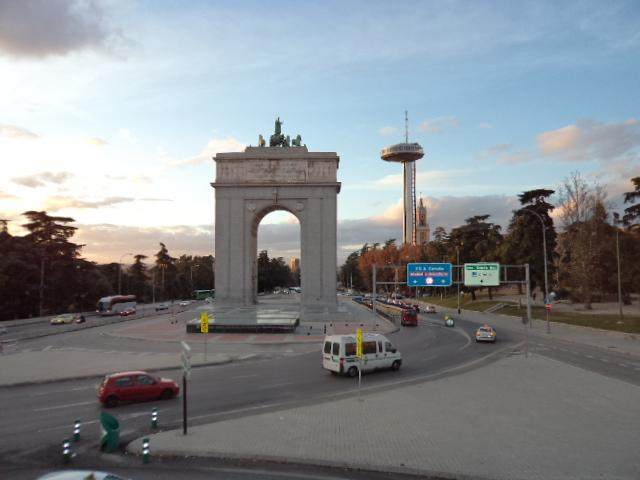
\includegraphics[scale=0.5]{Images/DSC00461}}
% \end{userstory}

% Esta es referencia a una tabla de historia de usuario \ref{tb:prueba}

% \begin{crccard}[tablacrc3]
% \crcclass{AlgoritmoGenetico}
% \crcresp
% {
% 	\begin{itemize}
% 	\item Crear el conjunto de genes necesarios para la creación de un individuo
% 	\item Realizar el proceso de mutación y recombinación
% 	\item Crear el conjunto de genes necesarios para la creación de un individuo
% 	\item Realizar el proceso de mutación y recombinación
% 	\end{itemize}
% }
% \crccolab
% {
% 	Población\\
% 	OperadorProbabilidad\\
% 	OperadorParejas\\
% 	OperadorReproducion\\
% 	Población
% }
% \end{crccard}

% \begin{crccard}[tablacrc2]
% \crcclass{AlgoritmoGenetico}
% \crcresp
% {
% 	\begin{itemize}
% 	\item Crear el conjunto de genes necesarios para la creación de un individuo
% 	\item Realizar el proceso de mutación y recombinación
% 	\item Crear el conjunto de genes necesarios para la creación de un individuo
% 	\item Realizar el proceso de mutación y recombinación
% 	\end{itemize}
% }
% \crccolab
% {
% 	Población\\
% 	OperadorProbabilidad\\
% 	OperadorParejas\\
% 	OperadorReproducion\\
% 	Población
% }
% \end{crccard}


% \begin{effortestimation}[tb:est1]
% 	\addentry[2]{Graficar secuencias de ensamble}{0.3} 
% 	\addentry[2]{Graficar secuencias de ensamble}{0.3} 
% 	\addentry[2]{Graficar secuencias de ensamble}{0.3} 
% 	\addentry[2]{Graficar secuencias de ensamble}{0.2}
% 	\addentry[2]{Graficar secuencias de ensamble}{0.2} 
% 	\addentry[4]{Graficar secuencias de ensamble}{0.1} 
% 	\addentry[4]{Graficar ensamble}{0.1} 
% 	\addentry[3]{Determinar Secuencia de Ensamble}{0.5} 
% 	\addentry[1]{Cargar Archivo}{0.8} 
% 	\addentry[1]{Determinar Secuencia de Ensamble}{0.2} 
% 	\addentry[1]{Gestionar restricción cambios de herramienta}{0.5} 
% 	\addentry[1]{Graficar secuencias de ensamble}{0.6} 
% \end{effortestimation}

% \begin{effortestimation}
% 	\addentry[4]{Graficar secuencias de ensamble}{1.1}  
% 	\addentry[3]{Determinar Secuencia de Ensamble}{2.5}  
% 	\addentry[2]{Graficar secuencias de ensamble}{0.3} 
% 	\addentry[2]{Graficar secuencias de ensamble}{0.3} 
% 	\addentry[2]{Graficar secuencias de ensamble}{0.2} 
% 	\addentry[2]{Graficar secuencias de ensamble}{0.2} 
% 	\addentry[1]{Cargar Fichero}{0.8} 
% 	\addentry[1]{Determinar Secuencia de Ensamble}{0.2} 
% 	\addentry[1]{Gestionar restricción cambios de herramienta}{0.5} 
% 	\addentry[1]{Esta es la prueba para el tinguiri}{0.5} 
% \end{effortestimation}

% Esto es una prueba de Tabla \ref{tb:est1}

% \begin{iterationplan}[tb:iterdurationtest]
% \setiterresult{1}{3} % in case an iteration takes a different time than the one calculated

% \end{iterationplan}

% %\geniterdurationplan[tb]{}

% Esto es una prueba de Tabla \ref{tb:iterdurationtest}

% \begin{engineeringtask}[tb:engtask]
% \engtaskuserstory{4}
% \engtaskname{Registrar usuario}
% \engtasktype{Registarse}
% \engtaskpointestimation{1}
% \engtaskstartdate{6}{5}{2014} % day, month, year
% \engtaskenddate{24}{10}{2014}
% \engtaskdescription{El usuario introduce sus datos para poder registrarse.}
% %\engtaskprogrammer{Alberto Medina Ramírez}
% \end{engineeringtask}

% \begin{developmenttask}[tb:devtask1]
% \devtaskuserstory{4}
% \devtaskname{Registrar usuario}
% \devtasktype{Registarse}
% \devtaskpointestimation{1}
% \devtaskstartdate{6}{5}{2014} % day, month, year
% \devtaskenddate{24}{10}{2014}
% \devtaskdescription{El usuario introduce sus datos para poder registrarse.}
% \devtaskprogrammer{Alberto Medina Ramírez}
% \end{developmenttask}

% \begin{developmenttask}[tb:devtask2]
% \devtaskuserstory{4}
% \devtaskname{Registrar usuario}
% \devtasktype{Registarse}
% \devtaskpointestimation{1}
% \devtaskstartdate{6}{5}{2014} % day, month, year
% \devtaskenddate{24}{10}{2014}
% \devtaskdescription{El usuario introduce sus datos para poder registrarse.}
% %\devtaskprogrammer{Alberto Medina Ramírez}
% \end{developmenttask}

% \begin{engineeringtask}[tb:engtask1]
% \engtaskuserstory{4}
% \engtaskname{Registrar usuario}
% \engtasktype{Registarse}
% \engtaskpointestimation{1}
% \engtaskstartdate{6}{1}{2014} % day, month, year
% \engtaskenddate{24}{11}{2014}
% \engtaskdescription{El usuario introduce sus datos para poder registrarse.}
% \engtaskprogrammer{Alberto Medina Ramírez}
% \end{engineeringtask}

% Referencia \ref{tb:devtask1}

% \begin{acceptancetest}[tb:expresult]
% \testcasecode{HU2\_P1}
% \testcasedescription{Prueba para la funcionalidad autentificar usuario.}
% \testcaseexeccond{
% El usuario debe estar previamente registrado.\\
% El usuario y contraseña deben ser válidos.
% }
% \testcaseexecstep{Se intenta autentificar un usuario en el sistema con los datos
% válidos.}
% \testcaseexpresult{El usuario se autentifica correctamente en el sistema.}
% \testcasename{Autentificar usuario en el sistema.}
% \testcaseuserstory{2}
% \end{acceptancetest}

% \begin{acceptancetest}[tb:expresultaa]
% \testcasecode{HU2\_P1}
% \testcasedescription{Prueba para la funcionalidad autentificar usuario.}
% \testcaseexeccond{
% El usuario debe estar previamente registrado.\\
% El usuario y contraseña deben ser válidos.
% }
% \testcaseexecstep{Se intenta autentificar un usuario en el sistema con los datos
% válidos.}
% \testcaseexpresult{El usuario se autentifica correctamente en el sistema.}
% \testcasename{Autentificar usuario en el sistema.}
% \testcaseuserstory{2}
% \end{acceptancetest}

% Prueba de link \ref{tb:expresult}